\documentclass[aspectratio=169,12pt]{beamer}
\usepackage{amsmath}
\usepackage{amssymb}
\usepackage{array}
\usepackage[most]{tcolorbox}
\usepackage{graphicx}
\usepackage{tikz}
\usepackage[sfdefault,lf]{FiraSans}
\renewcommand{\familydefault}{\sfdefault}
\setlength{\parindent}{0pt}
\everymath{\displaystyle}
\setbeamertemplate{navigation symbols}{}
\setbeamertemplate{footline}{}
\setbeamertemplate{headline}{}
\definecolor{mmpageWhite}{HTML}{FCFBF7}
\definecolor{mmtanSoft}{HTML}{F7F5EF}
\definecolor{mmgreenDeep}{HTML}{244B2C}
\definecolor{mmgreenLeaf}{HTML}{5D8A56}
\definecolor{mmgreenSoft}{HTML}{E4EFD9}
\definecolor{mmtext}{HTML}{163221}
\definecolor{mmwarn}{HTML}{8F2F36}
\definecolor{mmwarnSoft}{HTML}{F8E8EA}
\setbeamercolor{background canvas}{bg=mmpageWhite}
\setbeamercolor{normal text}{fg=mmtext,bg=mmpageWhite}
\newtcolorbox{MMCard}[2][]{enhanced,breakable=false,colback=#2,colframe=black,boxrule=1.5pt,arc=8pt,left=5pt,right=5pt,top=4pt,bottom=4pt,before skip=0pt,after skip=0pt,#1}
\newcommand{\KoruIcon}{\raisebox{-0.2em}{\includegraphics[height=1.05em]{../../../manamaths/SITE/header-logo.png}}}
\newcommand{\NotesTitle}[1]{{\colorbox{mmtanSoft}{\parbox{0.975\linewidth}{\vspace{0.14em}\hspace{0.25em}{\LARGE\bfseries\textcolor{mmgreenDeep}{#1}\hfill\KoruIcon}\vspace{0.14em}}}\par\vspace{0.18em}{\color{mmgreenLeaf}\rule{\linewidth}{2.0pt}}\par\vspace{0.12em}}}
\newcommand{\SectionTitle}[1]{{\large\bfseries\textcolor{mmgreenDeep}{#1}}\par\vspace{0.04em}}
\newcommand{\GreenDivider}{\par\vspace{0.01em}{\color{mmgreenLeaf}\rule{\linewidth}{2.4pt}}\par\vspace{0.03em}}
\newcommand{\KeyIdea}[1]{\begin{MMCard}[title={\textbf{Key idea}},colbacktitle=mmgreenSoft,coltitle=mmgreenDeep]{mmtanSoft}\small #1\end{MMCard}}
\newcommand{\WorkedExample}[2]{\begin{MMCard}[title={\textbf{#1}},colbacktitle=mmgreenSoft,coltitle=mmgreenDeep]{white}\small #2\end{MMCard}}
\newcommand{\CommonMistake}[1]{\begin{MMCard}[title={\textbf{Common mistake}},colbacktitle=mmwarnSoft,coltitle=mmwarn]{white}\small #1\end{MMCard}}
\newcommand{\TryThese}[1]{\begin{MMCard}[title={\textbf{Try these}},colbacktitle=mmgreenSoft,coltitle=mmgreenDeep]{mmtanSoft}\small #1\end{MMCard}}
\newcommand{\StepLine}[2]{\textbf{#1.} #2\par\vspace{0.03em}}

\setbeamertemplate{background}{
 \begin{tikzpicture}[remember picture,overlay]
 \draw[black,line width=1.5pt,rounded corners=10pt]
 ([xshift=0.45cm,yshift=-0.45cm]current page.north west)
 rectangle
 ([xshift=-0.45cm,yshift=0.45cm]current page.south east);
 \end{tikzpicture}
}
\begin{document}

\begin{frame}[t,shrink=12]
\NotesTitle{Notes \& Steps}
\footnotesize
\KeyIdea{Isometric drawing shows 3D objects on flat paper. Vertical lines stay vertical, but horizontal lines are drawn at 30$^\circ$ to the horizontal. Use isometric dot paper to keep proportions correct.}
\vspace{-0.3em}
\begin{columns}[T,onlytextwidth]
\begin{column}{0.48\textwidth}
\SectionTitle{Steps to draw a cube}
\StepLine{1}{Start at a dot. Draw a vertical line for the height.}
\StepLine{2}{From the bottom, draw a line up-right at 30$^\circ$ for the width.}
\StepLine{3}{From the bottom, draw a line up-left at 30$^\circ$ for the depth.}
\StepLine{4}{Complete the three visible faces using parallel lines.}
\StepLine{5}{Add dashed lines for hidden edges (optional).}
\end{column}
\begin{column}{0.48\textwidth}
\SectionTitle{Counting cubes}
\vspace{-0.2em}
\begin{center}
\scalebox{0.65}{
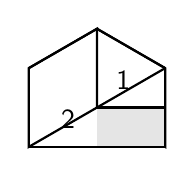
\begin{tikzpicture}
\draw[thick] (0,0)--(0.866,0.5)--(0.866,1.5)--(0,1)--cycle;
\draw[thick] (0.866,0.5)--(1.732,0)--(1.732,1)--(0.866,1.5);
\draw[thick] (0,0)--(0.866,0)--(1.732,0);
\draw[thick] (0,1)--(0.866,1.5)--(1.732,1);
\draw[thick] (0.866,0.5)--(1.732,1);
\draw[thick,fill=gray!20] (0.866,0)--(1.732,0)--(1.732,0.5)--(0.866,0.5);
\node at (1.2,0.85) {1};
\node at (0.5,0.35) {2};
\end{tikzpicture}
}
\end{center}
\vspace{-0.3em}
Count each cube including hidden ones. The drawing shows 2 cubes: one on top, one underneath on the right.
\end{column}
\end{columns}
\GreenDivider
\CommonMistake{Drawing horizontal lines as truly horizontal instead of at 30$^\circ$. In isometric, no line is truly horizontal except the base dots.}
\end{frame}

\begin{frame}[t,shrink=14]
\NotesTitle{Notes \& Steps}
\vspace{-0.3em}
\begin{columns}[T,onlytextwidth]
\begin{column}{0.48\textwidth}
\WorkedExample{Example 1: Drawing a cube}{
Draw a cube of side 2 units on isometric paper.
\vspace{0.3em}

Start with a vertical line of 2 units. From the bottom point, draw two lines at 30$^\circ$ of length 2 units each (one up-right, one up-left). Complete the three visible faces. Add hidden edges as dashed lines if needed.
}
\vspace{0.5em}
\WorkedExample{Example 2: Counting cubes}{
An isometric drawing shows a shape with visible cubes in a 2$\times$2$\times$1 arrangement (bottom layer of 4) plus 2 cubes on top of one corner. Total = 6 cubes.}
\end{column}
\begin{column}{0.48\textwidth}
\WorkedExample{Example 3: L-shape}{
An L-shaped solid has 3 cubes on the bottom row and 2 stacked on the leftmost cube. That's 5 cubes total: 3 base + 2 on top.}
\vspace{0.3em}
\TryThese{\begin{enumerate}
  \item Draw a single cube on isometric paper.
  \item How many cubes in a 2$\times$2$\times$2 cube? (answer: 8)
  \item Draw an L-shape of 3 cubes.
\end{enumerate}}
\end{column}
\end{columns}
\GreenDivider
\CommonMistake{Forgetting hidden cubes when counting. A 2$\times$2$\times$2 cube has 8 total but only 7 visible from most angles. Always account for all layers.}
\end{frame}

\end{document}
